\begin{figure}[t]
\centering
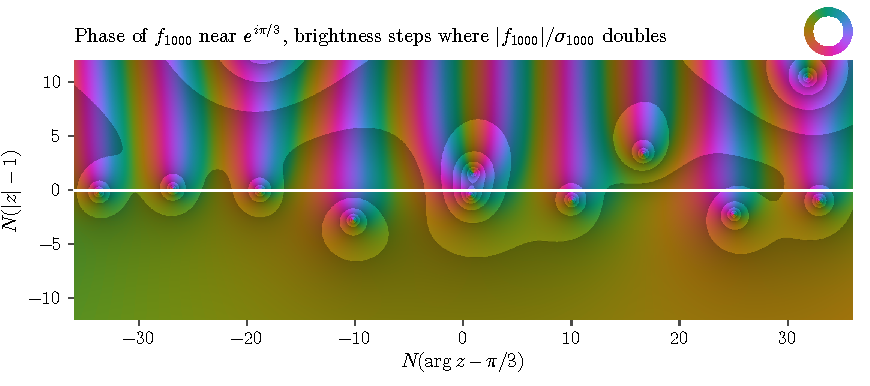
\includegraphics[width=0.85\textwidth]{figures/explanatory/phase-portrait.pdf}
\caption{Phase portrait of $f_{1000}$ near $e^{i\pi/3}$ for the sequence of
Figure~\ref{fig:root-matching}: the hue is $\arg f_{1000}$, all hues meet
at each zero, the brightness steps where $|f_{1000}|/\sigma_{1000}(|z|)$
doubles, and the white line is the unit circle. Near a zero with a large
derivative, $f_{1000}$ is nearly linear, so the small level curves are
nearly circles about it, like the boundaries of the disjoint disks about
the selected roots in Lemma~\ref{lem:isolation-interface}.}
\label{fig:phase-portrait}
\end{figure}
